\section{Sprint  Overview}\label{sec:SprintOverview}
The Senior Design I development methodology was an agile development methodology.
The features and milestones were created at the beginning of the semester.
Development sprints had a lifespan of two weeks each.
Each sprint began with a set of features and tasks that were to be accomplished during the two week sprint period.
These features and tasks were comprised of new items that needed to be completed in order to stay on track with the development schedule, as well as previous items that were not completed in the prior sprints.
At the beginning and end of each sprint, the development team would hold a sprint planning or a sprint retrospective meeting to discuss productivity and planning.\\

At the start of the Senior Design II course, the development team opted to use a Feature Driven Development (FDD) methodology.  
This decision was made primarily due to the large team size, scheduling meeting times for sprint planning and retrospective presented a challenge, as did the more rigid of the Agile methodology. 
The FDD schedule proved to be more flexible and efficient for such a large team with vastly different schedules between all of the members.  
This schedule also made it simple for the development team to branch into two individual sub-teams, each consisting of three members.  
One team that would work on creating an Android mobile application, and one team that would continue website and HoloLens development.

Suggested date ranges were still applied to each pending task. However, dates were much more flexible with this FDD system, it was mostly a method to ensure that the development team did not fall behind on completing the tasks.


\section{Sprint Schedule}
As stated above, the sprint cycles for Senior Design I were to be two weeks long. Each sprint was designed to accomplish a milestone, or set of related tasks. Below is the schedule of the sprints and what was accomplished during that time.

\begin{itemize}
	\item 9/18/2017   - Define milestones and user stories.
	\item 10/2/2017   - Base website created with file upload ability.
	\item 10/16/2017  - Wire frames, Presentation 1 documents, standalone file conversion.
	\item 10/30/2017  - File upload/download, file conversion integrated.
	\item 11/13/2017  - QR code generation, standalone advanced file conversion.
	\item 11/27/2017  - File conversion integration, create users, Presentation 2 documents.
	\item 12/04/2017  - Finish documentation, second semester preparation.
	\item 12/13/2017  - MVP delivered to sponsor.
	\item 04/27/2017  - Final product delivered to sponsor.
\end{itemize}

As stated above, the Senior Design II project management methodology switched from an Agile methodology to a Feature Driven Development methodology.  
This no longer held a rigid schedule for task deadlines and frequent meetings.
Instead, tasks were simply posted and worked on in a more free-form manner until they were completed. 
The tasks for Senior Design II were as follows:

	\begin{itemize}
		\item Website:
		\begin{itemize}
			\item Switch from the Azure Student free trial account to a Pay-As-You-Go subscription.
			\item Fully integrate the QR Code generator throughout the web application.
			\item Implement Microsoft Identity and Entity Framework as the application user management and DataBase providers.
			\item User profile creation and management through the web application interface.
			\item Implement Azure Blob Storage and structure patterns for user cloud file storage.
			\item Integrate web services with the mobile Android application.
			\item Explore web application security options (TLS).
			\item Refine the User Interface.
			\item Testing and documentation.
		\end{itemize}

		\item HoloLens:
		\begin{itemize}
			\item Create a custom Unity application capable of the following:
				\begin{itemize}
					\item Have an interactive user interface capable of utilizing common HoloLens gesture commands.
					\item Scan QR codes within the application.
					\item Retrieve 3D files from the web application by scanning QR codes.
					\item Render 3D models into the Unity application at runtime by scanning QR codes.
					\item Allow users to manipulate the rendered models in real-time.
				\end{itemize}
			\item Development on this application was abandoned due to an update to the HoloLens default 3D viewer application that covered all previously listed requirements.
		\end{itemize}

		\item Mobile Application:
		\begin{itemize}
			\item Determine the development platform and technology.
			\item Begin the application with ARCore package integration.
			\item Request and set appropriate user permissions on the device.
			\item Download 3D files by scanning QR codes within the application.
			\item Website integration:
			\begin{itemize}
				\item User login and authentication token retrieval.
				\item Listing files that the authenticated user has access to.
				\item Allowing selective download of available files without a QR code.
			\end{itemize}
			\item Refine the user interface.
			\item Testing and documentation.
		\end{itemize}
	\end{itemize}

\section{Timeline}
Below is the timeline of accomplished milestones.

\begin{figure}[H]
\begin{center}
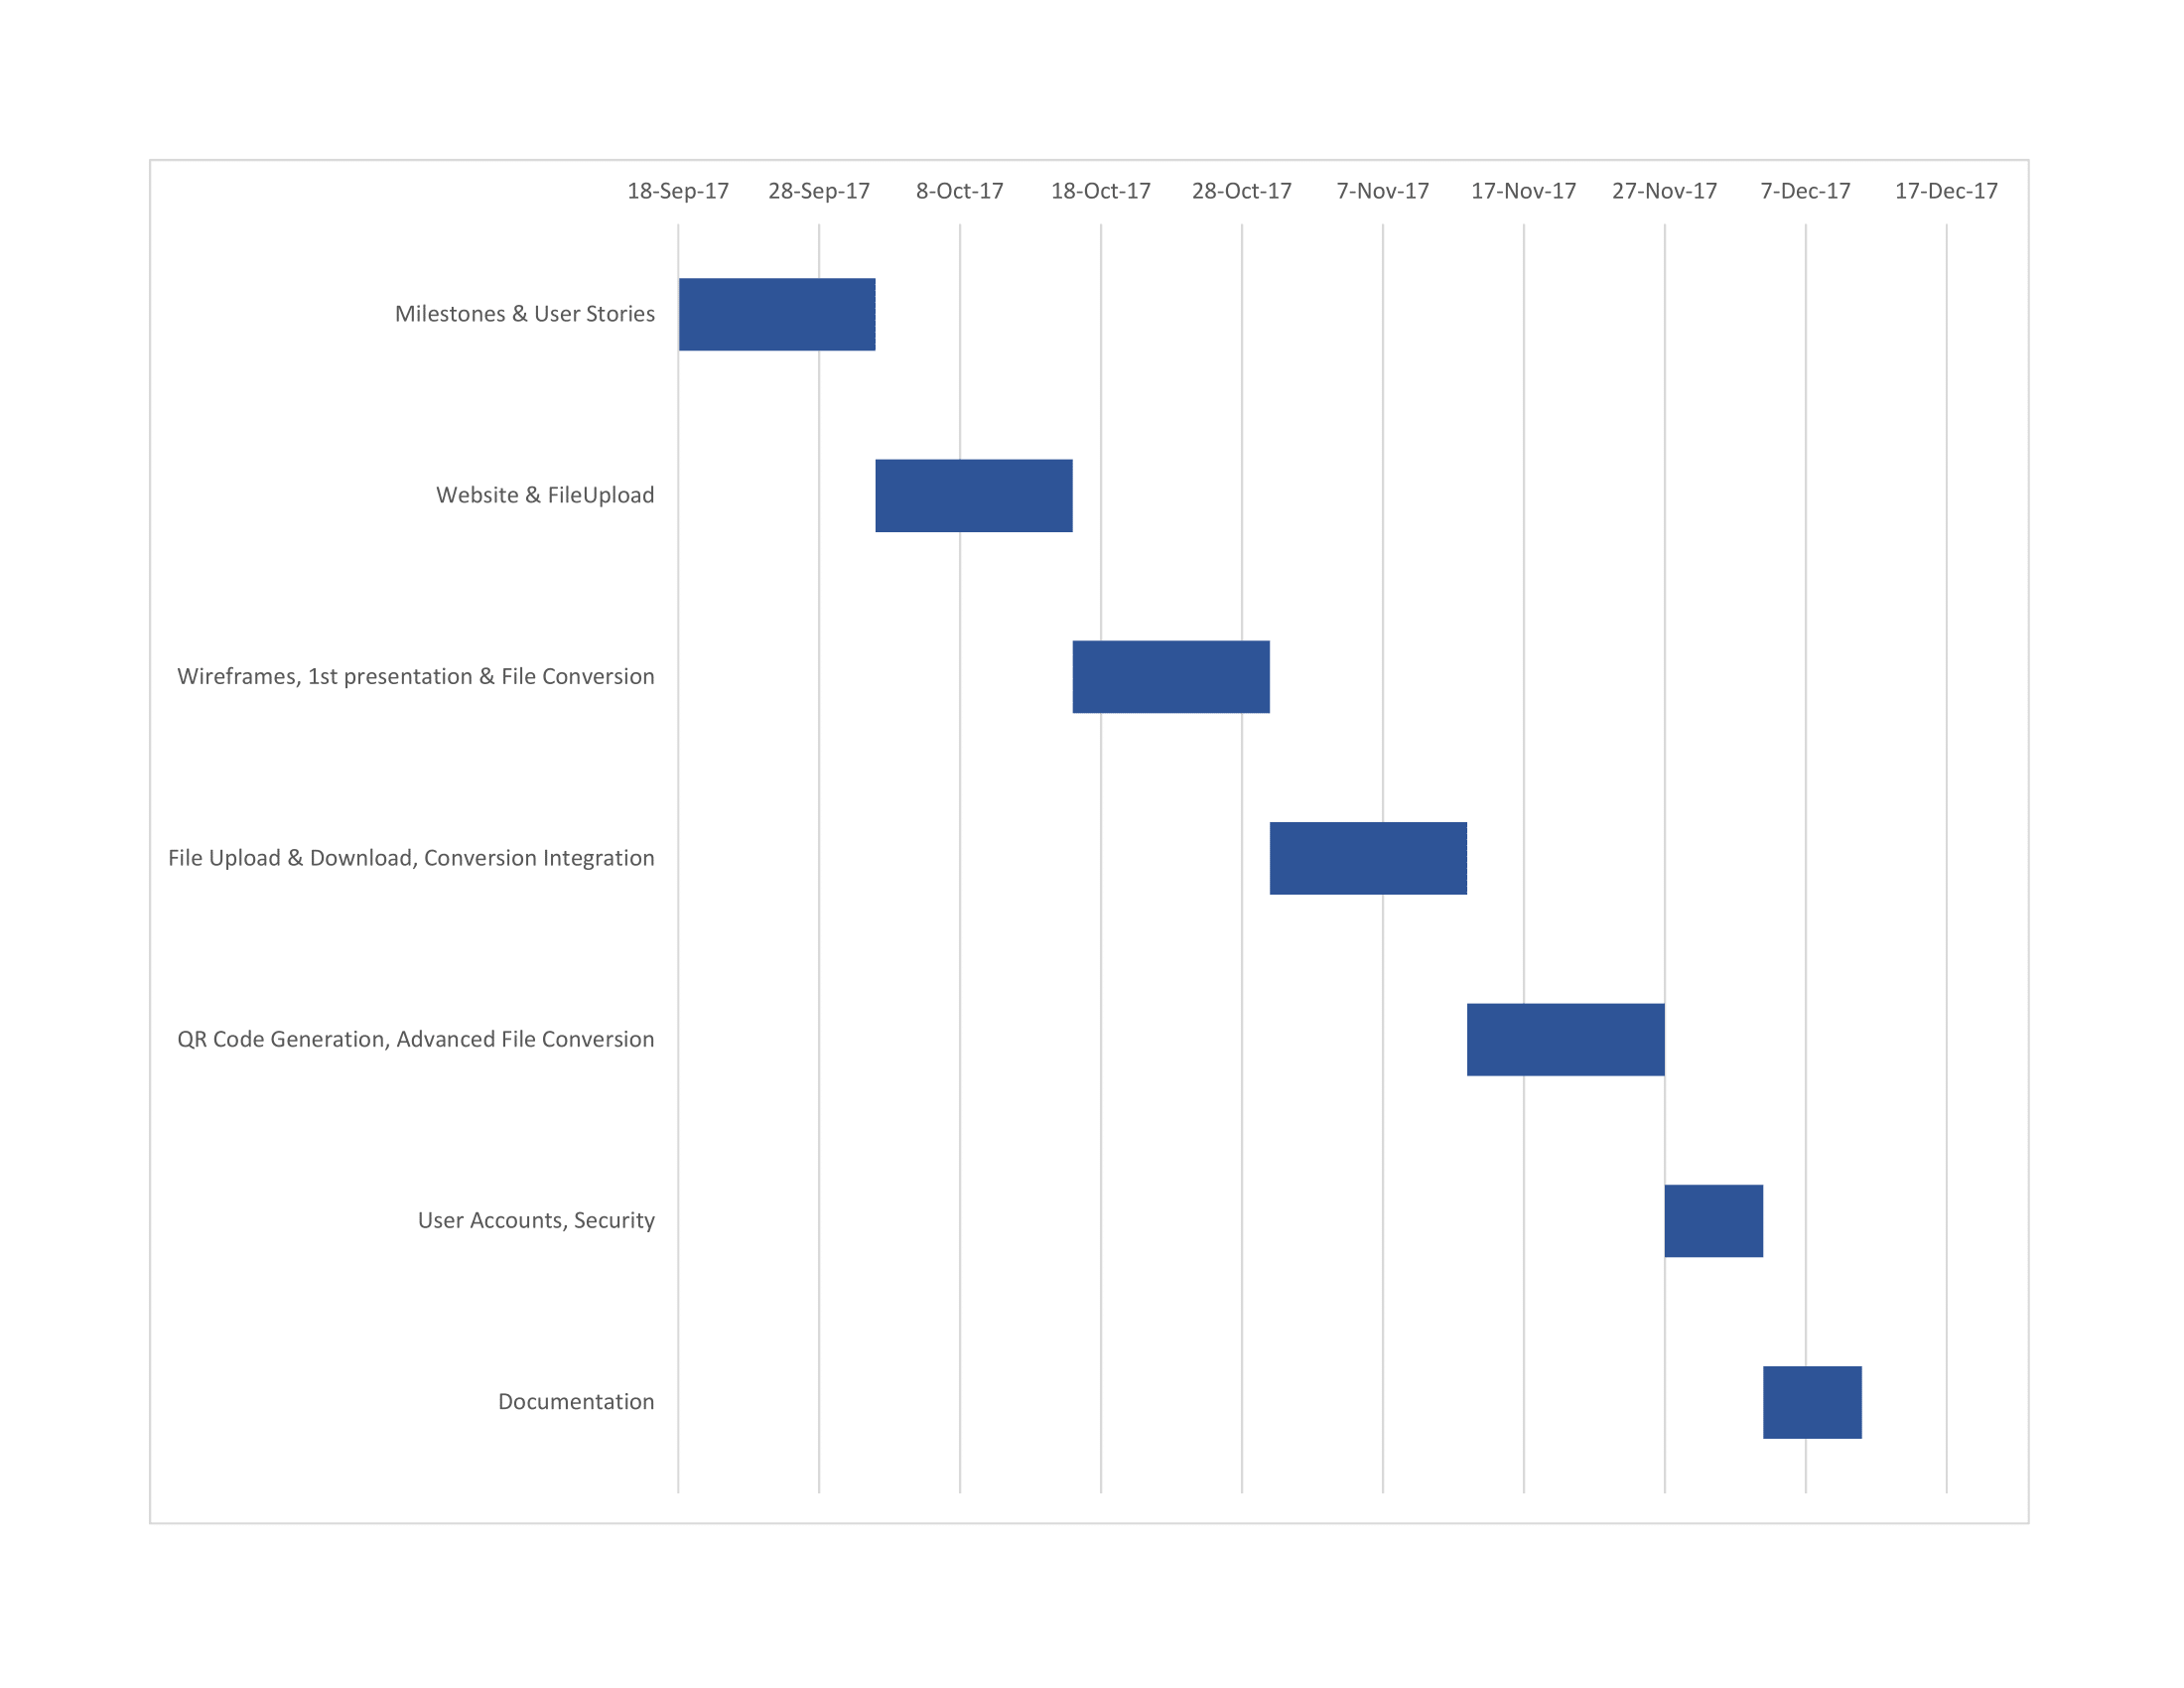
\includegraphics[width=1\textwidth]{./SprintGanattChart}
\end{center}
\caption{Sprint Timeline}
\end{figure}
